\section{Examples and visualization figures}

This appendix collects qualitative terminology visualizations copied into
\texttt{docs/paper/figures/}. They are included as debugging and explanation artifacts, not as final
quantitative results.

The refiner-highlight figures use three underline lanes: gray for all extracted candidate terms,
blue for terms selected by the domain-specific LLM refiner, and green for refined terms that also
have external verifier evidence.

\begin{figure}[htbp]
  \centering
  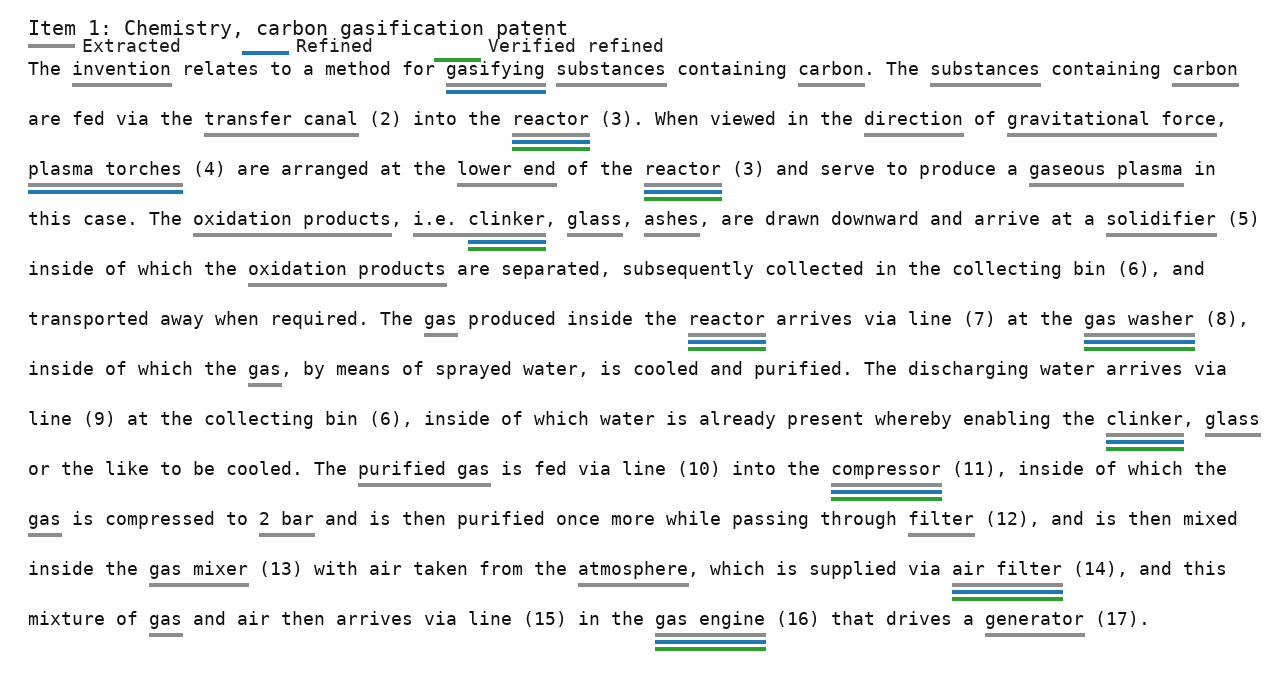
\includegraphics[width=\linewidth]{../figures/final-four-item-1-refiner-highlights.png}
  \caption{Chemistry patent example on carbon gasification.}
\end{figure}

\begin{figure}[htbp]
  \centering
  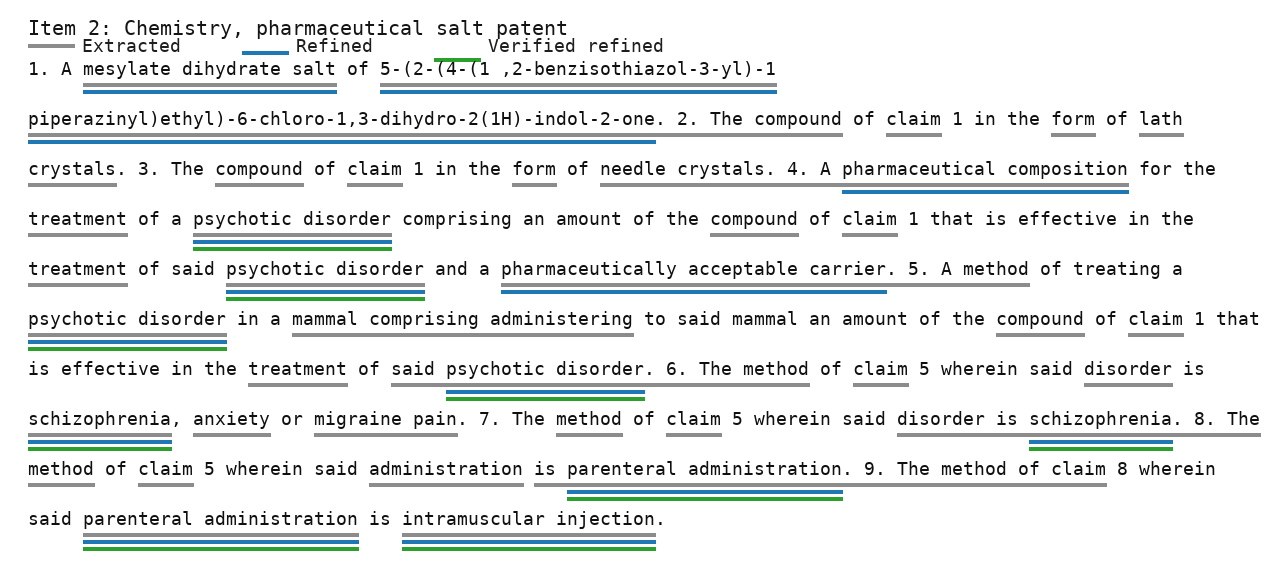
\includegraphics[width=\linewidth]{../figures/final-four-item-2-refiner-highlights.png}
  \caption{Chemistry patent example on pharmaceutical salts and formulation terminology.}
\end{figure}

\begin{figure}[htbp]
  \centering
  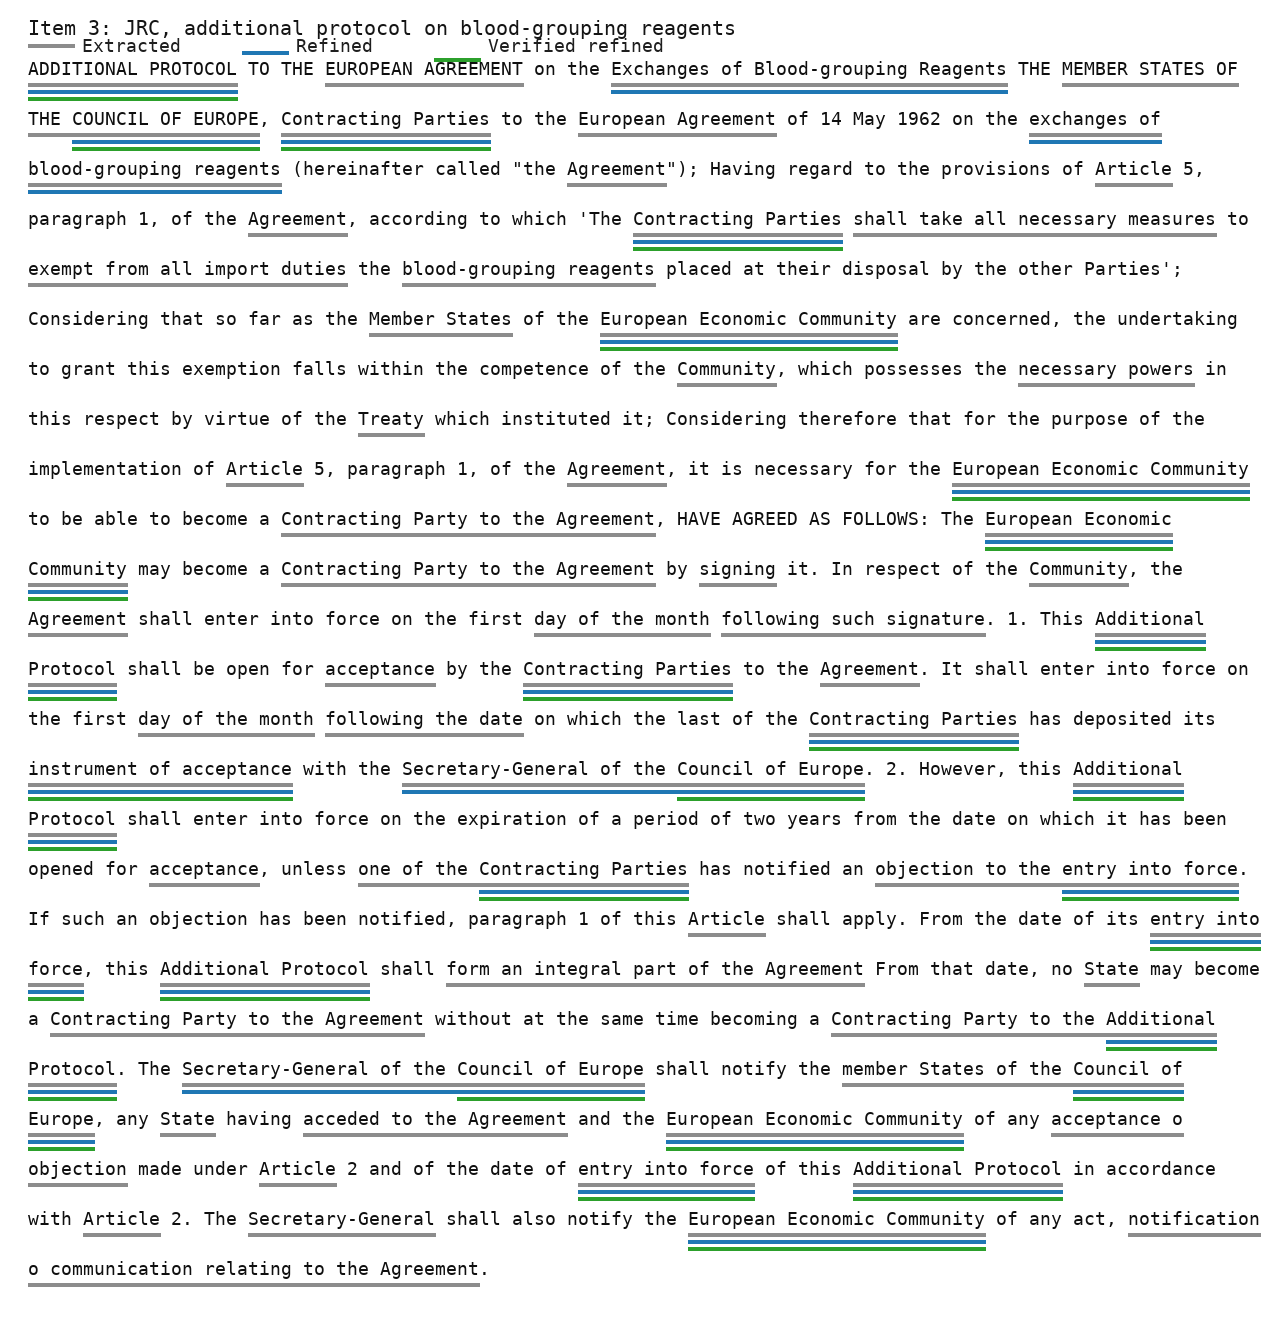
\includegraphics[width=\linewidth]{../figures/final-four-item-3-refiner-highlights.png}
  \caption{JRC legal example on blood-grouping reagents.}
\end{figure}

\begin{figure}[htbp]
  \centering
  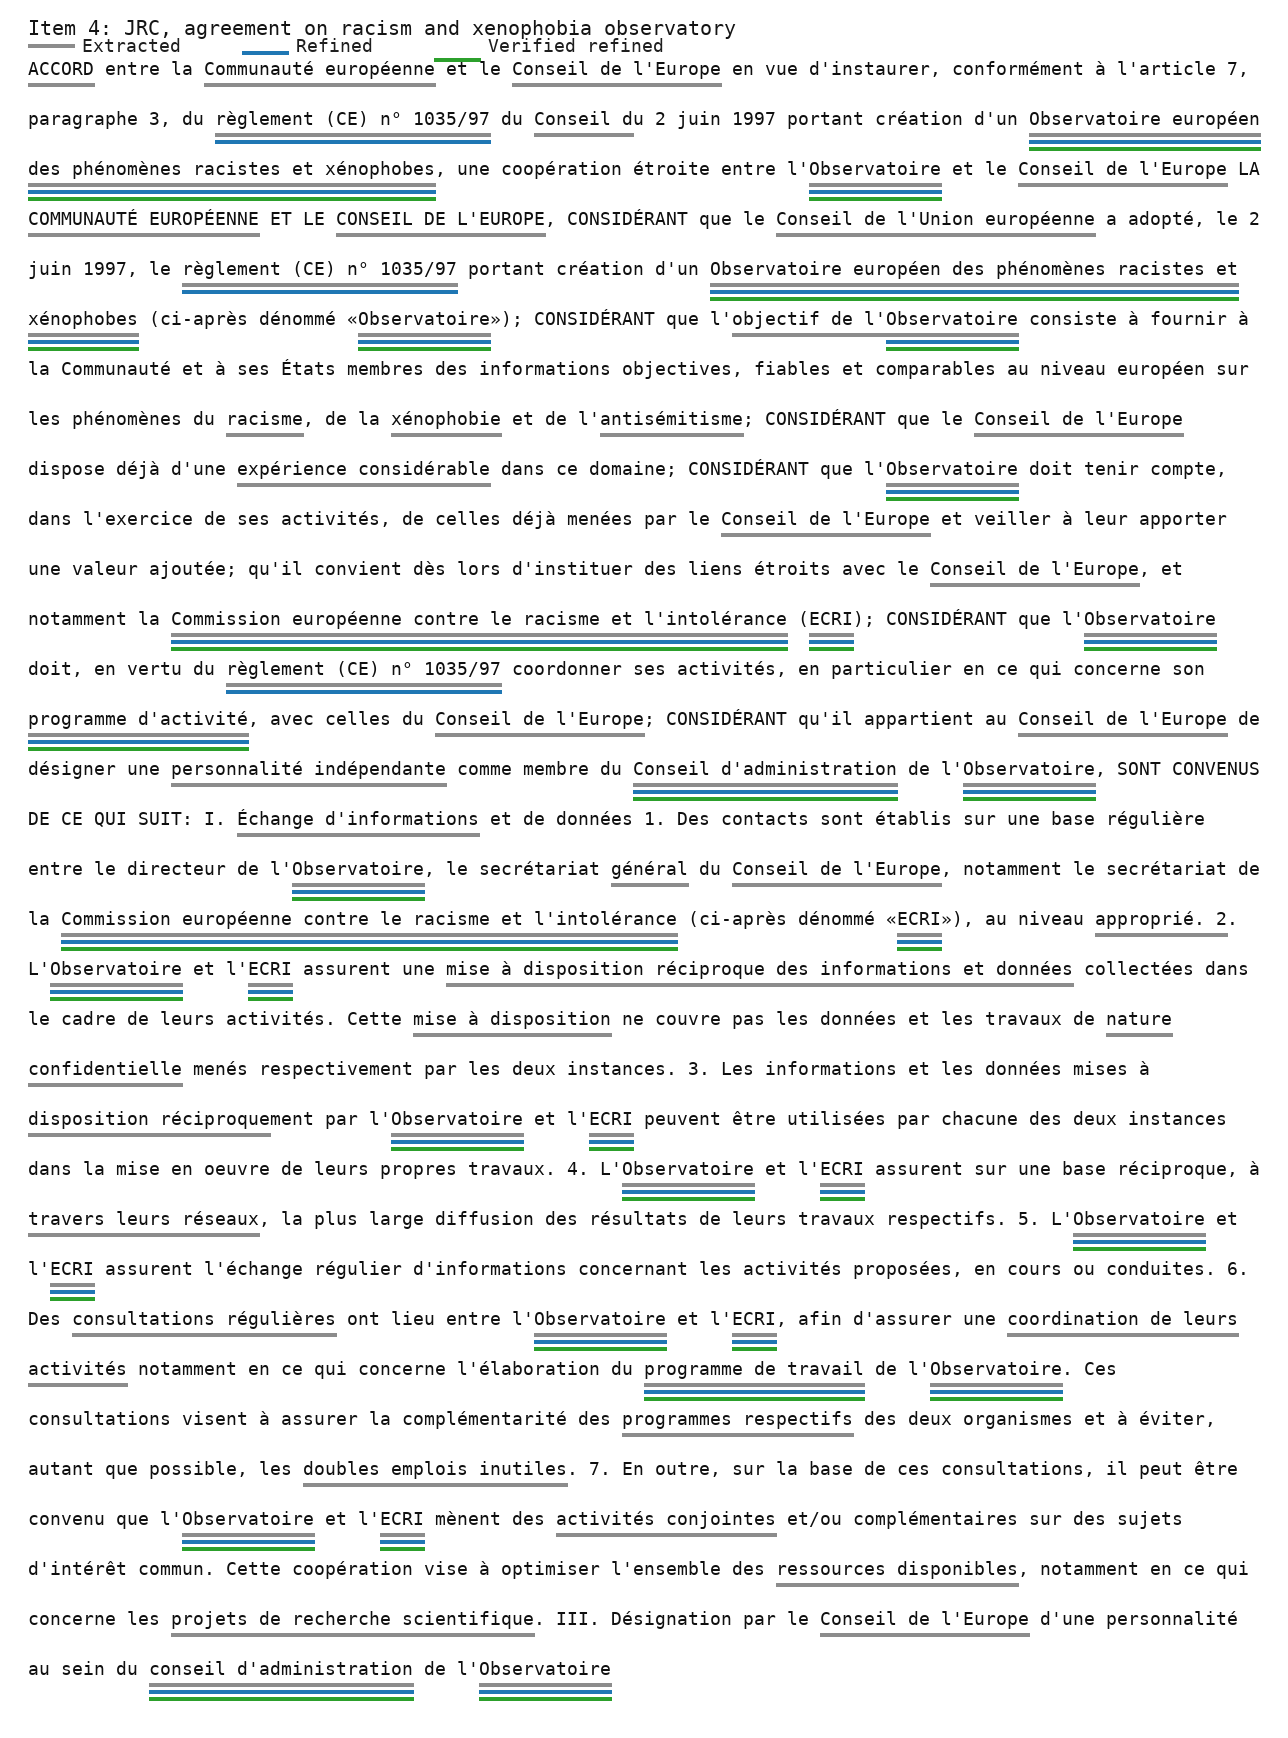
\includegraphics[width=\linewidth]{../figures/final-four-item-4-refiner-highlights.png}
  \caption{JRC legal example on the racism and xenophobia observatory.}
\end{figure}

\begin{figure}[htbp]
  \centering
  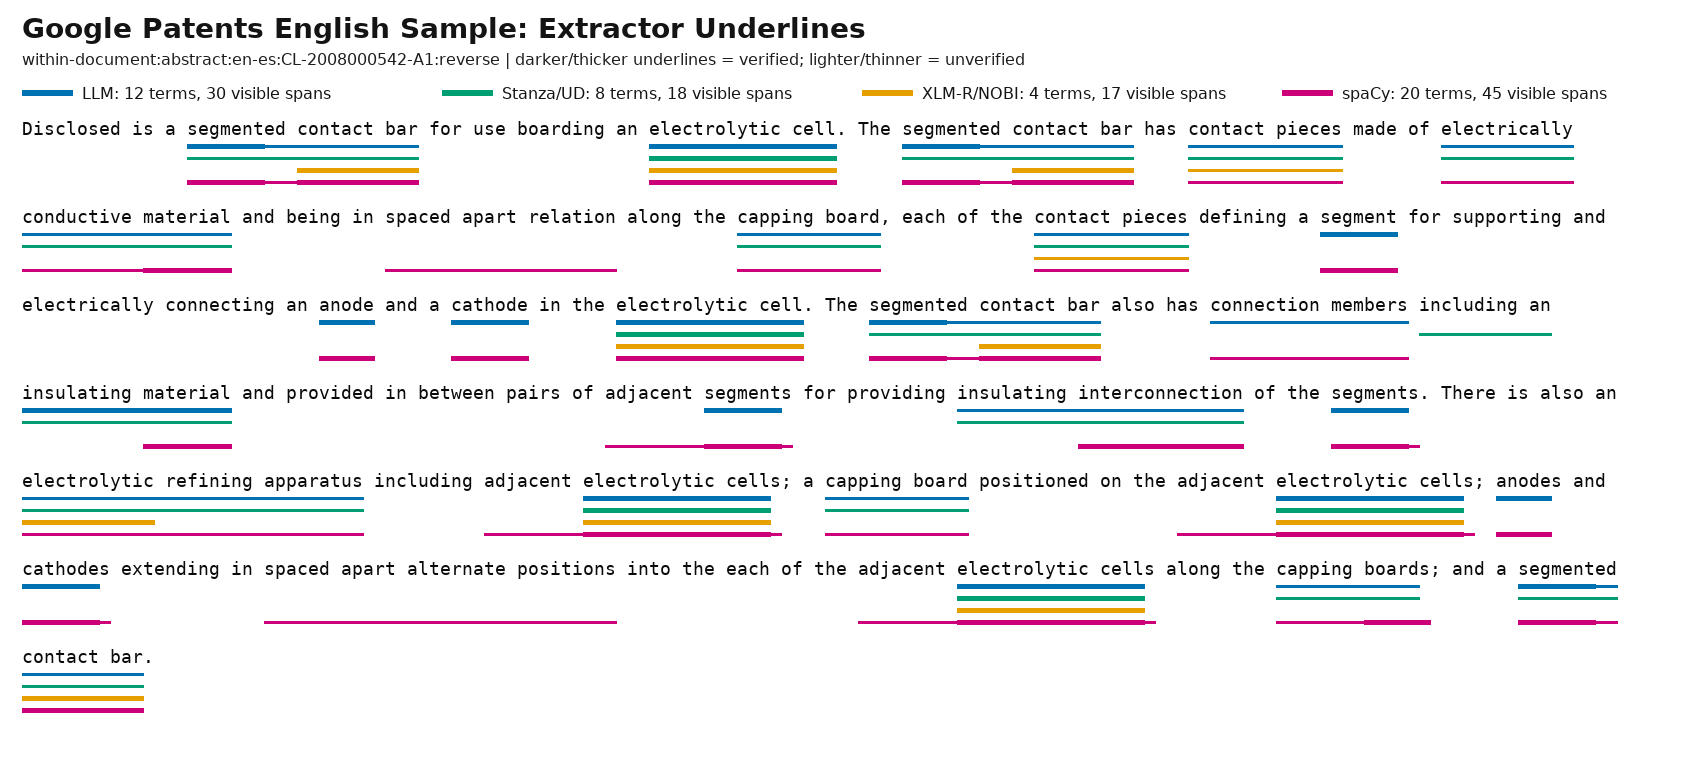
\includegraphics[width=\linewidth]{../figures/google-patents-english-extractor-highlights.png}
  \caption{Google Patents English extractor diagnostic visualization.}
\end{figure}

\begin{figure}[htbp]
  \centering
  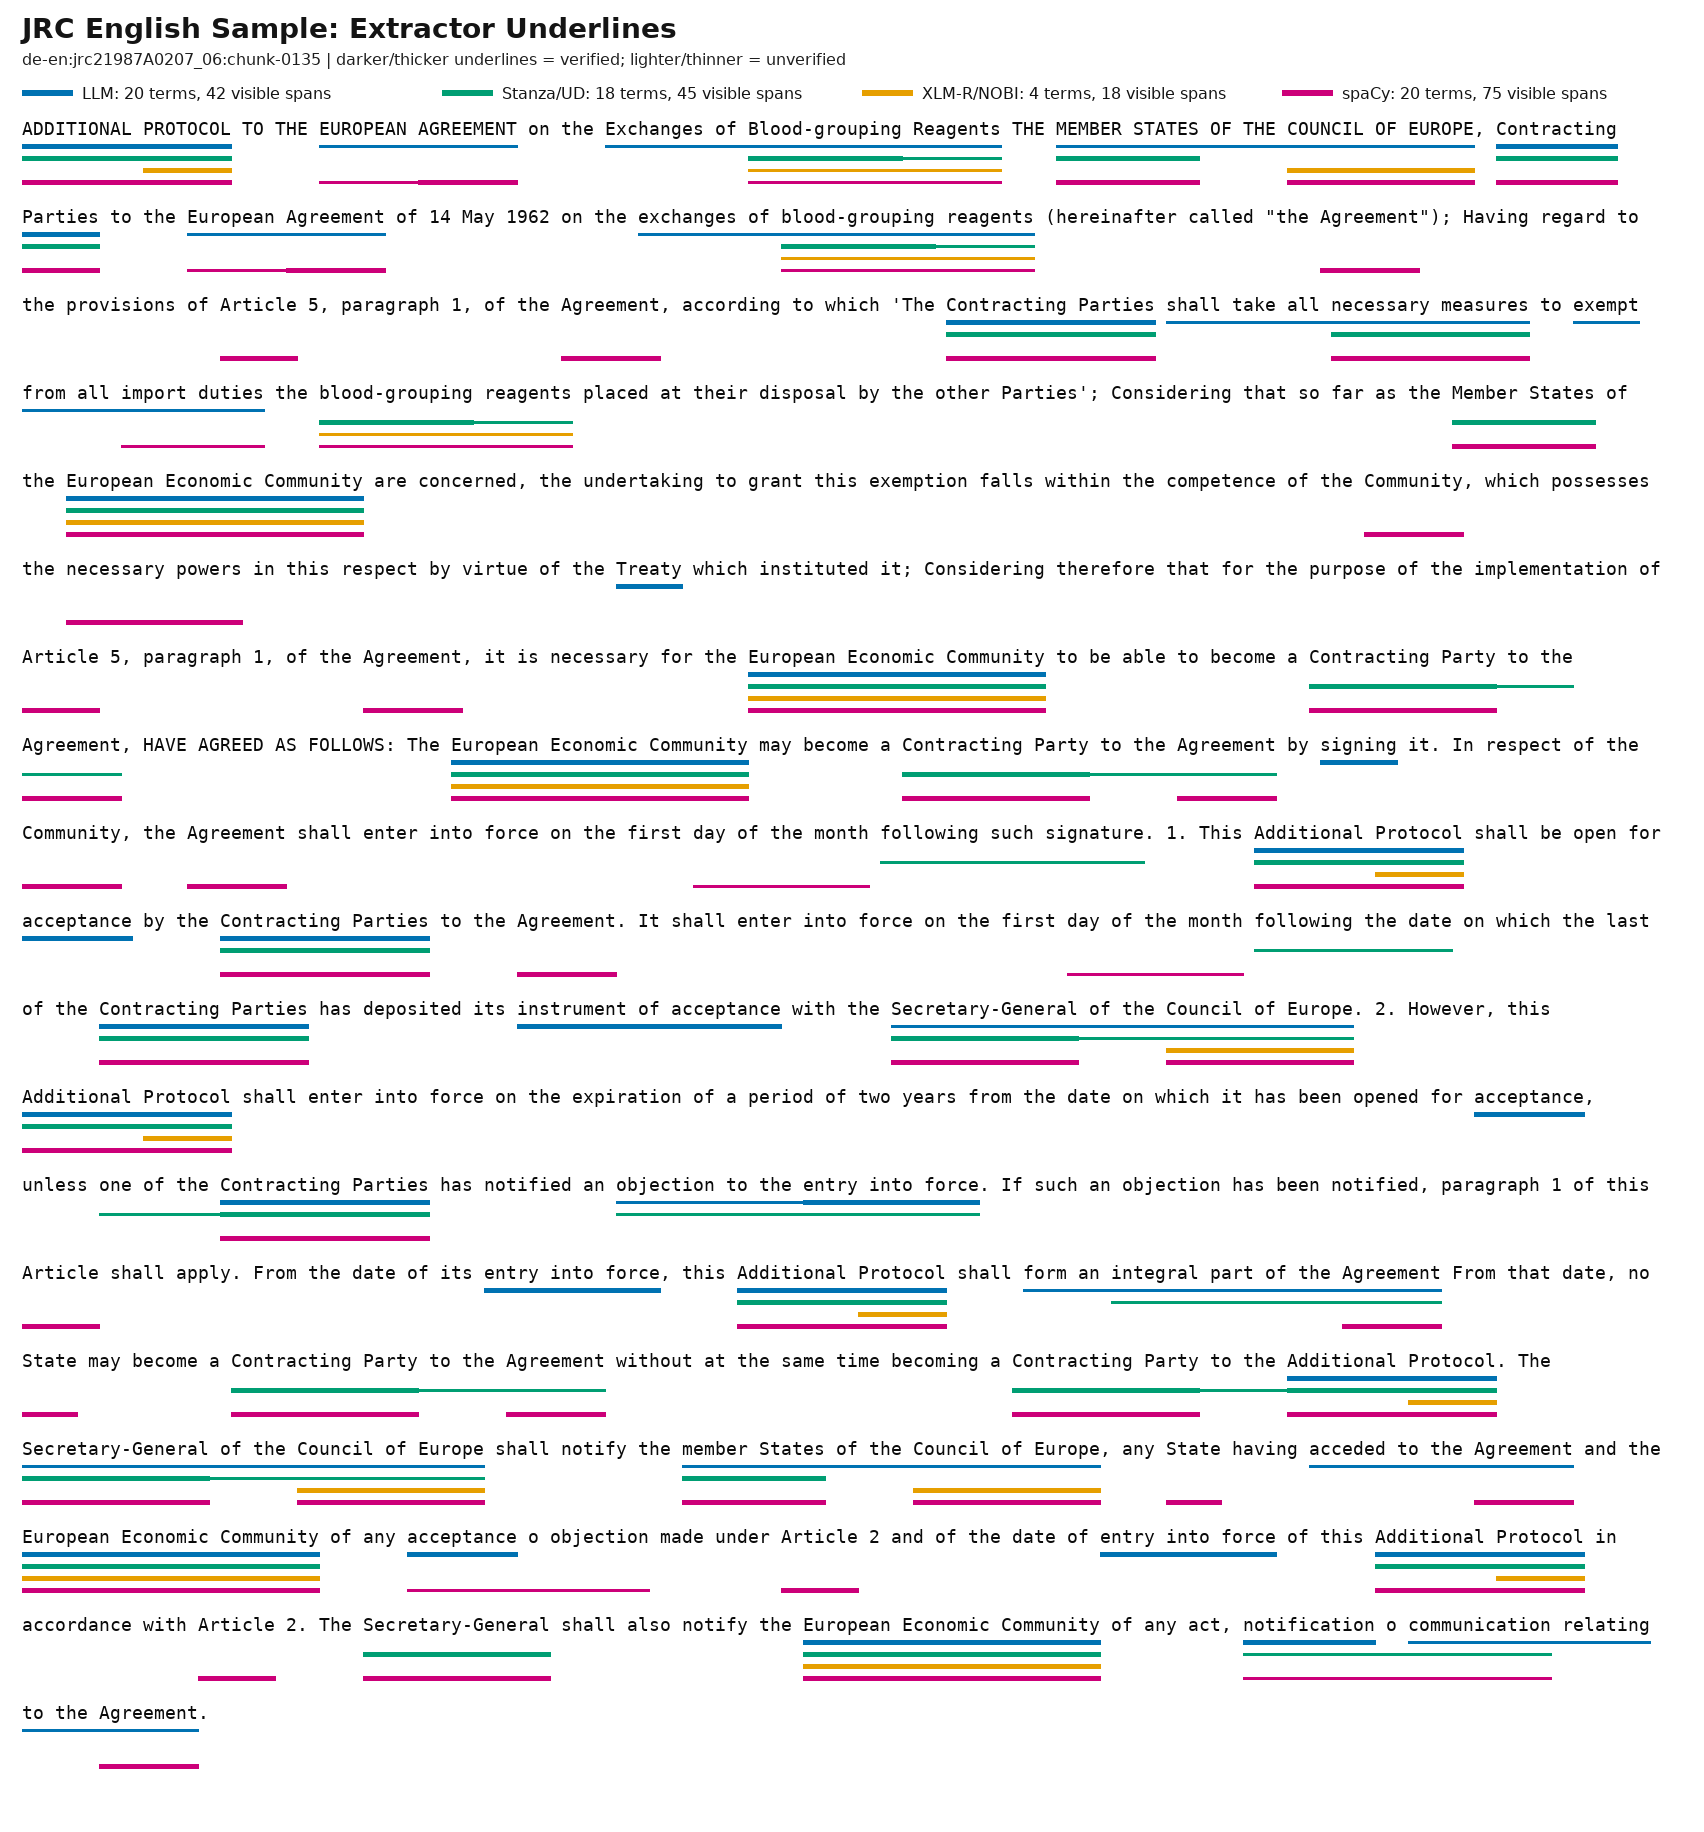
\includegraphics[width=\linewidth]{../figures/jrc-english-extractor-highlights.png}
  \caption{JRC English extractor diagnostic visualization.}
\end{figure}
